%!TEX root = ../thesis.tex
\section{Service: Entwurf und Implementierung}

\subsection{Elixir und Phoenix}

Bei Webanwendungen hängt (wie in anderen Domänen auch) die Wahl einer Programmiersprache des Webservices weniger davon ab, welches Problem die Anwendung lösen soll, sondern mehr von den Erfahrungen der im Projekt beteiligten Entwickler ab. Die Auswahl an serverseitigen Programmiersprachen ist groß, und jede Programmiersprache besitzt ihre eigenen Vorteile.

Die Wahl der Programmiersprache fiel für dieses Projekt auf \textbf{Elixir}.

Elixir wurde 2011 von José Valim veröffentlicht und ist somit eine relativ junge Programmiersprache. Elixir basiert jedoch auf Erlang, einer seit 1986 von Ericsson entwickelten Programmiersprache und Laufzeitumgebung. Das Erlang System ist u.a. für seine hohe Verfügbarkeit bekannt, es kann auf vielen Servern parallel laufen und aktualisiert werden, ohne die Anwendung stoppen zu müssen. Die Programmiersprache Erlang ist funktional, weshalb Elixir ebenfalls eine funktionale Programmiersprache ist.

Elixir wurde nicht gewählt, da darin schon Erfahrung besteht, sondern um Erfahrung in Elixir zu erlangen: Zu Beginn der Arbeit waren weder Kenntnisse in Elixir noch in Erlang vorhanden.

Als Webframework für Elixir wurde das bekannteste Framework gewählt: \textbf{Phoenix}.

Phoenix ist ein Framework für Webanwendungen nach dem \ac{MVC} Modell. Es beinhaltet viele nützliche Bestandteile wie eine Datenbank-Abstraktion (ähnlich zu einem \acs{ORM}\footnote{\acf{ORM}; da Elixir eine funktionale Programmiersprache ist und somit keine Objekte besitzt, ist der Begriff \acs{ORM} nicht zutreffend, jedoch vergleichbar mit ORMs aus anderen Sprachen.}) und eine einfache Implementierung von Websockets, welche im weiteren Verlauf der Arbeit zur Echtzeitkommunikation benötigt werden.

\subsection{Entwurf einer RESTful API}

\ac{REST} ist ein von Roy Fielding entworfener Architekturstil für \emph{``verteilte Hypermedia Systeme''}. Fielding nennt grundlegend zwei Bedingungen für ein solches System:

\begin{itemize}
  \item Die Trennung des Systems in eine Client-Server Architektur. Dies folgt dem Prinzip der ``Trennung der Belange'' \emph{(Separation of Concern)} in das Belangen der Nutzeroberflächer (Client) und das Belangen der Datenverwaltung (Server).
  \item Die Kommunikation zwischen Client und Server ist zustandslos \emph{(stateless)}. Der Client muss dem Server alle Daten übermitteln, die der Server zum Verständnis und Ausführen der Anfrage benötigt.\footnote{Im Gegensatz zu Sessions, bei denen auf dem Server Informationen zu jedem Client gespeichert werden.}
\end{itemize}

Alle Interaktionen bestehen grundlegend aus einer Ressource, einem Identifikator und einer Aktion \citep[12]{Webber2010}. REST ist kein Standard, daher kann sich die Implementierung von REST\footnote{Wenn wir REST implementieren, verwenden wir die Adjektivform \emph{``RESTful''}.} von Fall zu Fall unterscheiden. Bei Webanwendungen werden meist mindestens folgende Informationen aus dem HTTP Protokol genutzt:

\begin{itemize}
  \item Der Pfad der URL bestimmt die Ressource und den Identifikator.
  \item Die HTTP Methode bestimmt die auszuführende Aktion.
\end{itemize}

In Richardsons Maturity Model entspricht dies einem Level Two Service (vgl. \citep[20]{Webber2010}). Dabei werden auch HTTP Statuscodes genutzt, um dem Client einen standardisierten Status der Anfrage zu übermitteln.

Für den Service wurden die in Tabelle \ref{tab:rest-routes} definierten Endpunkte für eine RESTful API ausgearbeitet. Als Datenformat soll JSON genutzt werden, was sich für die Verwendung in einem JavaScript-basierten Frontend Client eignet.

\begin{table}[H]
  \footnotesize
  \begin{tabularx}{\textwidth}{| l | l | X |}
    \hline
    \textbf{Verb} & \textbf{Pfad} & \textbf{Beschreibung} \\ \hline
    GET & {\scriptsize \texttt{/projects}} & Auflisten aller Projekte \\ \hline
    POST & {\scriptsize \texttt{/projects}} & Erstellen eines neuen Projekts \\ \hline
    GET & {\scriptsize \texttt{/projects/:project\_id}} & Auslesen eines Projekts anhand seiner ID \\ \hline
    PUT & {\scriptsize \texttt{/projects/:project\_id}} & Aktualisieren eines Projekts anhand seiner ID \\ \hline
    DELETE & {\scriptsize \texttt{/projects/:project\_id}} & Löschen eines Projekts anhand seiner ID \\ \hline
    GET & {\scriptsize \texttt{/projects/:project\_id/pipelines}} & Auflisten aller Pipelines in einem Projekt \\ \hline
    POST & {\scriptsize \texttt{/projects/:project\_id/pipelines}} & Erstellen einer neuen Pipeline in einem Projekt \\ \hline
    GET & {\scriptsize \texttt{/projects/:project\_id/builds}} & Auflisten der letzten Builds eines Projekts anhand seiner ID \\ \hline
    GET & {\scriptsize \texttt{/pipelines/:pipeline\_id}} & Auslesen einer Pipeline anhand ihrer ID \\ \hline
    PUT & {\scriptsize \texttt{/pipelines/:pipeline\_id}} & Aktualisieren einer Pipeline anhand ihrer ID \\ \hline
    DELETE & {\scriptsize \texttt{/pipelines/:pipeline\_id}} & Löschen einer Pipeline anhand ihrer ID \\ \hline
    GET & {\scriptsize \texttt{/pipelines/:pipeline\_id/builds}} & Auflisten der letzten Builds einer Pipeline anhand ihrer ID \\ \hline
    GET & {\scriptsize \texttt{/builds/:build\_id}} & Auslesen eines Builds anhand seiner ID \\
    \hline\hline
    POST & {\scriptsize \texttt{/webhooks/receive}} & Endpunkt für Git Webhooks mit verschiedenen Aktionen, bspw. Erstellen eines neuen Builds\footnote{Diese Route entspricht nicht einer typischen RESTful Route, wird allerdings für das Empfangen von Webhooks auf diese benötigt} \\
    \hline
  \end{tabularx}
  \caption{RESTful API Routen}
  \label{tab:rest-routes}
\end{table}

\subsection{Die ``JSON API'' Spezifikation}
\label{subsec:jsonapi}

Zum Entwurf einer API im JSON Datenformat gibt es u.a. die Spezifikation ``JSON API''. Diese Spezifikation beinhaltet viele Konventionen zu den Daten, die zur API bzw. von der API gesendet werden.

Durch das Befolgen dieser Spezifikation lässt sich ein Level Three Service nach Richardsons Maturity Model implementieren (vgl. \citep[20]{Webber2010}): Durch eingebettete Links zu anderen Ressourcen wird die Bedingung des \emph{Hypermedia as the Engine of Application State (HATEOAS)} erfüllt.

Es ist jedoch sehr aufwändig die gesamte JSON API Spezifikation zu implementieren. Daher wurde sich zur Implementierung auf die Top Level Struktur\footnote{vgl. http://jsonapi.org/format/\#document-top-level} beschränkt. Diese besitzt drei Teile:

\begin{itemize}
  \item \texttt{data} beinhaltet alle Daten der Ressource.
  \item \texttt{error} beinhaltet alle Fehler, die durch die Anfrage entstanden sind.
  \item \texttt{meta} beinhaltet optionale Informationen zur Anfrage.
\end{itemize}

\lstinputlisting
  [caption={Vereinfachte Struktur der JSON API Ausgabe},
  label={lst:jsonapi-simple-example}]
  {snippets/jsonapi-example.json}

\subsection{RESTful API in Phoenix}

Die Implementierung der RESTful API besteht in Phoenix aus:

\begin{enumerate}
  \item Konfiguration der Routen
  \item Erstellen eines Controllers mit zu den Routen passenden Methoden
  \item Erstellen eines Views zur Ausgabe
\end{enumerate}

Im Folgenden wird dieser Prozess anhand der Ressource für Pipelines erklärt.

\subsubsection{Konfiguration der Routen}

Zur Konfiguration der Routen stellt Phoenix die Datei \texttt{router.ex} bereit. Darin können Routen über anhand einer HTTP Methode, einem Pfad, einem Modul und der darin enthaltenen Funktion definiert werden.

\lstinputlisting
  [caption={Phoenix Router mit HTTP Methoden},
  label={lst:router-http-verbs},
  language=elixir]
  {snippets/pipeline-routes-long.ex}

Phoenix besitzt ebenfalls die Funktion \texttt{resource()}\footnote{In Elixir können Klammern von Funktionen auch ausgelassen werden.} anstatt der HTTP Methode, welche alle Routen für eine REST Ressource erstellt. Diese Funktion lässt sich konfigurieren, um nur bestimmte Routen für eine Ressource zu erstellen oder auch um weitere Routen in einer Ressource zu erstellen.

Die Definitionen aus Quelltext \ref{lst:router-http-verbs} lassen sich damit folgendermaßen umstrukturieren:

\lstinputlisting
  [caption={Phoenix Router mit REST Ressourcen},
  label={lst:router-resources},
  language=elixir]
  {snippets/pipeline-routes.ex}

Die Ressource für Projekte besitzt in Quelltext \ref{lst:router-resources} durch \texttt{only: []} keine eigenen Routen und erscheint daher überflüssig. Dies soll jedoch nur als Beispiel für verschachtelte Ressourcen dienen. Im finalen Router besitzt die Projekt-Ressource selbstverständlich auch eigene Routen.

\subsubsection{Erstellen eines Controllers}

Ein Controller ist ein Modul mit den im Router definierten Funktionen (vgl. Quelltext \ref{lst:router-http-verbs} und \ref{lst:router-resources}). Demnach werden folgende Funktionen für den \texttt{PipelineController} benötigt:

\begin{itemize}
  \item \texttt{index} zur Auflistung der Pipelines.
  \item \texttt{create} zum Erstellen einer Pipeline.
  \item \texttt{show} zur Ausgabe einer Pipeline.
  \item \texttt{update} zum Bearbeiten einer Pipeline.
  \item \texttt{delete} zum Löschen einer Pipeline.
\end{itemize}

In den Funktionen eines Controllers werden meist Datenbankabfragen und -operationen durchgeführt. In einer Funktion kann auch direkt auf die Datenbank zugegriffen werden, jedoch nutzt Phoenix das Entwurfsmuster der ``Contexts''.

Bei Contexts handelt es sich um kein ausgefallenes Entwurfsmuster. Es beschreibt nur, dass zusammengehörigen Funktionen in einem Modul gruppiert werden sollen. Datenbankabfragen und -operationen für eine Ressource sind zusammengehörige Funktionen, und werden daher in einem Context zusammengefasst. In Quelltext \ref{lst:pipeline-controller} werden zwei Contexts genutzt: \texttt{Warp.Pipelines} und \texttt{Warp.Projects}.

\lstinputlisting
  [caption={Phoenix Controller für die Pipeline Ressource},
  label={lst:pipeline-controller},
  language=elixir]
  {snippets/pipeline-controller.ex}

Üblicherweise besteht eine Funktion eines Controllers zuerst aus Datenbankabfragen und -operationen und danach aus einer darauf bezogenen Antwort.

In Zeilen 24 bis 33 des Controllers (Quelltext \ref{lst:pipeline-controller}) ist zu sehen, wie je nach Erfolg oder Misserfolg der Funktion \texttt{Pipelines.create()} unterschiedliche Antworten ausgegeben werden.

Beachtenswert sind auch die Funktionsaufrufe, deren Funktionsname mit einem Ausrufezeichen enden. Solche Funktionen können unter Umständen einen Fehler werfen. In Zeile 12 (Quelltext \ref{lst:pipeline-controller}) wird die Funktion \texttt{Projects\allowbreak.get!()} aufgerufen, um ein Projekt anhand seiner ID abzufragen. Sollte kein Projekt mit dieser ID gefunden werden, wirft diese Funktion einen Fehler. Phoenix kann diesen Fehler korrekt interpretieren und antwortet automatisch mit einer entsprechenden Fehlermeldung. Auf diese Weise können auch eigene Fehler implementiert werden.\footnote{vgl. https://hexdocs.pm/phoenix/errors.html}

Die Antwort wird über die Funktion \texttt{render()} gesendet, die einen zugehörigen View aufruft.

\subsubsection{Erstellen eines Views}

Views sind in Phoenix dazu zuständig, eine Antwort in einem beliebigen Format wie HTML, XML oder JSON auszugeben. Wir nutzen letzteres Format, JSON, zur Implementierung einer API im JSON-Format.

Phoenix transformiert einen Elixir-Hash als Ausgabe im View automatisch zu einem JSON-Objekt. Im View wird folglich nur ein Hash zurückgegeben.

\lstinputlisting
  [caption={Phoenix View für die Pipeline Ressource},
  label={lst:pipeline-view},
  language=elixir]
  {snippets/pipeline-view.ex}

Um eine einzige Ressource oder eine Liste von Ressourcen zurückzugeben, stellt Phoenix die Funktionen \texttt{render\_one} und \texttt{render\_many} bereit. In Zeile 5 und 9 (Quelltext \ref{lst:pipeline-view}) ist ebenso ersichtlich, dass die Daten der Ressource in dem JSON API Top Level Teil \texttt{data} ausgegeben werden (vgl. Kapitel \ref{subsec:jsonapi}).

\subsubsection{Nutzung der angelegten API Routen}
\label{subsec:api-usage}

Im Folgenden werden die angelegten API Routen zur Verifizierung der Funktionalität und als Beispiel zur Nutzung aufgerufen. Dazu wird das \ac{CLI} \texttt{curl} genutzt. Im Vorfeld wurde ein Projekt mit der ID 1 angelegt.

Da noch keine Pipelines angelegt wurden, wird bei der Auflistung der Pipelines eine leere Liste zurückgegeben.

\lstinputlisting
  [caption={API Beispiel: Auflistung aller Pipelines ohne angelegte Pipelines}]
  {snippets/api-example-get-pipelines.txt}

Um weitere Operationen auf einer Pipeline ausführen zu können, wird zunächst eine Pipeline angelegt.

\lstinputlisting
  [caption={API Beispiel: Anlegen einer Pipeline}]
  {snippets/api-example-create-pipeline.txt}

Zur Verifikation kann nochmals die Auflistung aller Pipelines aufgerufen werden. Als Ausgabe erhalten wir nun eine Liste mit einer Entität.

\lstinputlisting
  [caption={API Beispiel: Auflistung aller Pipelines mit angelegter Pipeline}]
  {snippets/api-example-get-pipelines-again.txt}

Die Attribute der Pipeline lassen sich alle zusammen oder einzeln bearbeiten. Um genau zu sein handelt es sich beim Aktualisieren einzelner Attribute um eine \texttt{PATCH} Anfrage. Dies wurde zur Vereinfachung und einfacheren Handhabung nicht berücksichtigt und unter \texttt{PUT} zusammengefasst.

\lstinputlisting
  [caption={API Beispiel: Aktualisierung einer Pipeline}]
  {snippets/api-example-update-pipeline.txt}

Sollten ungültige Attribute übergeben werden, wird – wie in der JSON API Spezifikation definiert (siehe Sektion \ref{subsec:jsonapi}) – eine passende Fehlermeldung ausgegeben. In Beispiel \ref{lst:api-example-update-error} wird zur Erzeugung eines Fehlers der Titel der Pipeline auf eine Nummer gesetzt.

\lstinputlisting
  [caption={API Beispiel: Ungültige Aktualisierung einer Pipeline},
  label={lst:api-example-update-error}]
  {snippets/api-example-update-pipeline-error.txt}

Zuletzt kann die Pipeline gelöscht werden. Als Bestätigung wird zusätzlich eine Nachricht ausgegeben.

\lstinputlisting
  [caption={API Beispiel: Löschen einer Pipeline}]
  {snippets/api-example-delete-pipeline.txt}

\subsection{Konfiguration einer Pipeline}

In den Beispielen aus Sektion \ref{subsec:api-usage} wurden bisher nur direkte Attribute einer Pipeline angelegt. Die Abschnitte und Schritte einer Pipeline (siehe Sektion \ref{subsec:uml}) wurden darüber allerdings nicht bewusst angelegt. Sie sollen nämlich aus einer Konfigurationsdatei ausgelesen werden.

Das Anlegen komplexer Pipelines mit mehreren Stages, Abschnitten und verschachtelten Abschnitten gestaltet sich über eine UI schwierig und hat schnell das Potential, lästig zu werden. Eine Konfigurationsdatei ist in solchen Fällen vorteilhafter und besonders bei Entwicklern beliebt. Ein sehr großer Vorteil ist, dass die Konfigurationsdatei direkt auch unter Versionskontrolle steht, wenn sie als Datei im Projekt angelegt ist.

Es wurde festgelegt, dass die Datei `.warp.yml` im Dokumentenstamm des Projekts vorhanden sein muss. Aus ihr wird der Aufbau der Pipeline ausgelesen und vor dem Starten des Build-Prozesses alle Abschnitte und Schritte in die Datenbank eingetragen.

In der Konfigurationsdatei können sich Konfigurationen für mehrere Pipelines befinden. Die zugehörige Pipeline wird über einen Identifikator bestimmt. (Vgl. \texttt{konfiguration\_\allowbreak inidentifikator} in Abbildung \ref{fig:uml} bzw. \texttt{human\_id} in der letztendlichen Implementation, vgl. Sektion \ref{subsec:api-usage})

Die Konfigurationsdatei ist im YAML-Format notiert. YAML\footnote{http://yaml.org/} ist ein menschenfreundlicher Standard. Beispielsweise besitzt JSON, was zur API-Kommunikation genutzt wird, im Gegensatz zu YAML keine Kommentare.

Quelltext \ref{lst:example-config} zeigt eine mögliche Konfiguration. Bei \texttt{steps\_\allowbreak parallel} und \texttt{steps\_\allowbreak serial} handelt es sich um die Abschnitte, deren Schritte entweder seriell oder parallel ausgeführt werden. In diesem Beispiel wird auch ersichtlich, wie sich mehrere Abschnitte ineinander verschachteln lassen.

\lstinputlisting
  [caption={Konfiguration einer Pipeline im YAML Format},
  label={lst:example-config}]
  {snippets/config-example-yml.yml}

Die Konfigurationsdatei enthält noch andere Besonderheiten, wie bspw. ein \texttt{include} Kennwort, mit dem Stages, Abschnitte und Schritte zwischen in mehreren Pipelines genutzt werden können. Auf weitere Besonderheiten und Implementierungen hierzu wird nicht weiter eingegangen.

\subsection{Ablauf eines Build-Prozesses}

Ein kompletter Build-Prozesses läuft in den folgenden Schritten ab, nachdem ein Git Webhook empfangen wurde:

\begin{description}
  \item[Schritt 1:] Die Anfrage auf Starten des Build-Prozesses wird in eine Warteschlage pro Pipeline gespeichert. Build-Prozesse der gleichen Pipeline sollen nicht gleichzeitig laufen.
  \item[Schritt 2:] Abarbeiten der Pipeline-Warteschlange.
  \item[Schritt 3:] Erstellen eines temporären Ordners, in dem der Build-Prozess ausgeführt wird.
  \item[Schritt 4:] \texttt{git clone} des Repositories in den temporären Ordner.
  \item[Schritt 5:] \texttt{git checkout} des Repositories an die im Webhook übertragene Stelle.
  \item[Schritt 6:] Auslesen der Konfigurationsdatei.
  \item[Schritt 7:] Abspeichern der Stages, Abschnitte und Schritte.
  \item[Schritt 8:] Ausführen des eigentlichen Build-Prozesses (\textbf{Build Worker}).
  \item[Schritt 9:] Darin wird die erste Stage ausgeführt (\textbf{Stage Worker}).
  \item[Schritt 10:] Darin werden Abschnitte oder Schritte ausgeführt, parallel oder seriell (\textbf{Group Worker} bzw. \textbf{Step Worker}).
  \item[Schritt 11:] Falls vorhanden, werden darin weitere verschachtelte Abschnitten oder Schritte ausgeführt (zurück zu Schritt 10).
  \item[Schritt 12:] Ausführen der nächsten Stage (zurück zu Schritt 9).
  \item[Schritt 13:] Wurden alle Stages ausgeführt, ist der Build Worker beendet.
  \item[Schritt 14:] Löschen des temporären Ordners.
\end{description}

Das Ausführen des eigentlichen Build-Prozesses (Schritte 8 bis 13) und dessen Abhängigkeiten zu anderen Workern lässt sich als Prozess grafisch verständlicher in einem vereinfachten Ablaufdiagramm (Abbildung \ref{fig:ablauf-build-prozess}) darstellen.

\begin{figure}[h]
  \caption{Vereinfachtes Ablaufdiagramm des Build-Prozesses}
  \label{fig:ablauf-build-prozess}
  \centering
    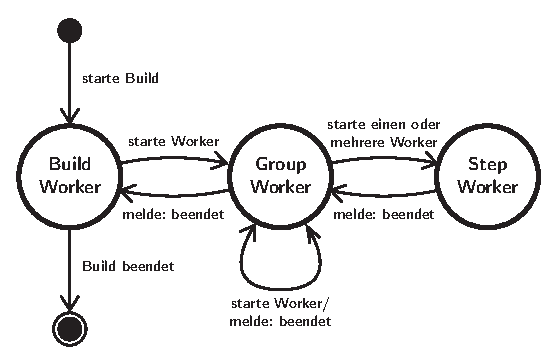
\includegraphics[width=\textwidth]{assets/worker_diagram}
\end{figure}

In Abbildung \ref{fig:ablauf-build-prozess} ist zu sehen, wie von links nach rechts der Ablauf des Build-Prozesses geleitet wird, bis ganz rechts jeweils ein \emph{Step Worker} den eigentlichen Befehl ausführt.

Verschachtelte Worker melden ihrem übergeordneten Worker, wenn sie ihre Arbeit beendet haben. Der übergeordnete Worker kann nun weitere Worker starten, oder selbst seinem übergeordneten Worker melden, dass er beendet ist. Die Abfolge findet also rein über Kommunikation zwischen den einzelnen Workern statt.

\subsection{Implementierung der Worker des Build-Prozesses}
